
	\section{Backend Server}\label{subsec_general_backend}
	 In principle the core of all tasks of the backend server is, to apply clustering methods to data (dataset and goldstandard) in an automatized and autonomous way, using only the configurations and inputs the user specified. The produced results have to be parsed in such a way, that the frontend can easily collect certain information and visualize them. Thus the components used by the backend that are not directly included into the framework programatically but need to be provided can be summarized as
	 \begin{itemize}
	 	\item Data (Datasets \& Goldstandards)
	 	\item Clustering Methods
	 	\item Configurations
	 \end{itemize}
	 
	 Additional components that can be extended and might be needed in case the provided standard functionality of the framework is not sufficient for the user

	\begin{itemize}
		\item Data input formats (including parsers)
		\item Run result formats (including parsers)
		\item Clustering Quality Measures
		\item Distance Measures
		\item Parameter Optimization Methods
		\item Dataset types
		\item (Data, Run \& Run-Data) Statistics
		\item Dataset generators
\end{itemize}		 
	 
	 All these components have to be located in the \textbf{repository} of the framework (see \ref{subsec_repository} for more details). The repository is a file system hierarchy located at a specified path and contains all components used by and available to the framework. Datasets, clustering methods or configurations outside the repository cannot be used by the framework.
	 
	 After these components have been made available to the backend, they can be combined almost arbitrarily. In the following we will describe the dependencies of each of these components which need to be fulfilled such that a new component of each type can be recognized and used by the framework.
	 

	\subsection{Repository}\label{subsec_repository}
		The backend server is based on a central repository which concludes all files in its folder structure. You can easily start a framework with a different set of files by simply using another repository.
		
		\begin{figure}[hbtp]
		\caption{Repository folder structure}
		\centering
		\includegraphics[width=\textwidth]{../master_seminar_presentation/repository_structure.png}
		\end{figure}
		

		\subsubsection{Repository folder structure}
			\begin{itemize}[noitemsep]
				\item \textbf{data}: Contains all data-related files.
				\begin{itemize}[noitemsep,nolistsep]
					\item \textbf{configs} [*.dataconfig]: Contains the data configuration files \ref{subsec:dataconfigs}.
					\item \textbf{datasets}: Contains all dataset-related files \ref{subsec:datasets}.
					\begin{itemize}[noitemsep,nolistsep]
						\item \textbf{configs} [*.dsconfig]: Contains the dataset configuration files \ref{subsubsec:datasetconfigs}.
						\item \textbf{[subfolder for every dataset]}: The dataset files themselves.
					\end{itemize}
					\item \textbf{goldstandards}: Contains all goldstandard-related files \ref{subsec:goldstandards}.
					\begin{itemize}[noitemsep,nolistsep]		
						\item \textbf{configs} [*.gsconfig]: Contains the goldstandard configurations \ref{subsubsec:gsconfigs}.
						\item \textbf{[subfolder for every goldstandard]}: Contains the goldstandard files themselves.
					\end{itemize}
				\end{itemize}
				\item \textbf{programs}: Contains all program-related files \ref{programs}.
				\begin{itemize}[noitemsep,nolistsep]
					\item \textbf{configs} [*.config]: Contains all program configuration files \ref{subsec_programconfigs}.
					\item \textbf{[subfolder for every program]}: The program files themselves.
				\end{itemize}
				\item \textbf{results}: The results of run executions \ref{runresults}.
				\begin{itemize}[noitemsep,nolistsep]
					\item \textbf{[subfolder for every run execution]}: A subfolder contains the results of one run execution.
					\begin{itemize}[noitemsep,nolistsep]
						\item \textbf{clusters}: The clustering results, including clustering qualities and graphics.
						\item \textbf{configs}: Copies of all used configuration files of this run execution to enable exact reproduction.
						\item \textbf{inputs}: Copies of all used inputs of this run execution to enable exact reproduction.
						\item \textbf{logs}: All log files corresponding to this run execution.
					\end{itemize}
				\end{itemize}
				\item \textbf{runs}: All run-related files \ref{sec:runs}.
				\begin{itemize}[noitemsep,nolistsep]
					\item \textbf{[*.run: a file for every run]}: Contains the run-files.
				\end{itemize}
				\item \textbf{supp}: Contains supplementary material.
				\begin{itemize}[noitemsep,nolistsep]
					\item \textbf{clustering}: Supplementary material related to clusterings.
					\begin{itemize}[noitemsep,nolistsep]
						\item \textbf{paramOptimization}: Contains clustering parameter optimization methods \ref{paramOptMethods}.
						\begin{itemize}[noitemsep,nolistsep]
							\item \textbf{[*.jar]}: Each jar-file corresponds to a parameter optimization method and is loaded dynamically by the framework.
						\end{itemize}
						\item \textbf{qualityMeasures}: Contains clustering quality measures \ref{clustQualMeasures}.
						\begin{itemize}[noitemsep,nolistsep]
							\item \textbf{[*.jar]}: Each jar-file corresponds to a clustering quality measure and is loaded dynamically by the framework.
						\end{itemize}
					\end{itemize}
					\item \textbf{formats}: Contains all formats used by the framework.
					\begin{itemize}[noitemsep,nolistsep]
						\item \textbf{dataset}: Contains all dataset formats \ref{formats}.
						\begin{itemize}[noitemsep,nolistsep]
							\item \textbf{[*.jar]}: Each jar-file corresponds to a dataset format and is loaded dynamically by the framework.
						\end{itemize}
						\item \textbf{runresult}: Contains all runresult formats \ref{formats}.
						\begin{itemize}[noitemsep,nolistsep]
							\item \textbf{[*.jar]}: Each jar-file corresponds to a runresult format and is loaded dynamically by the framework.
						\end{itemize}
					\end{itemize}
				\end{itemize}
			\end{itemize}
	 
	 \subsection{Clustering Methods}\label{programs}
	 Clustering Methods (technically also called \textbf{Programs} throughout this guide) can be executed by the framework, and be applied to data to calculate clusterings.
	 In order to include a new clustering method and use it within the framework, 
	\begin{itemize}		
		\item the \textbf{executable} of the method has to be made available to the framework (an exception are Clustering Methods provided through the R framework, see \ref{rprograms}), 
		\item the method itself has to be specified in a configuration file (called \textbf{program configuration})
		\item all other components (e.g. \textbf{input} and \textbf{output formats}) specified in the program configuration need to be available.
\end{itemize}
The configuration file for a clustering method (short \textbf{program configuration}) contains all information required, such that the framework can execute the method in an automatized and autonomous way. These information include for example, among others, the name of the method, its supported input formats, its output format, its parameters (including type and valid range of values). An exact description of how program configurations look like and which options and settings need to be specified can be found in \ref{subsec_programconfigs}.
	
	\clusteval ships with a set of clustering methods including
	\begin{itemize}
		\item Affinity Propagation
		\item Hierarchical Clustering$^{(Rserve)}$
		\item K-Means$^{(Rserve)}$
		\item Markov Clustering
		\item Spectral Clustering$^{(Rserve)}$
		\item Transitivity Clustering
	\end{itemize}
	
	For every of these clustering methods a \textbf{program configuration} is also provided, such that they are directly usable from the start. Of course these program configurations can be modified and adapted to the user's needs.
	
	\subsubsection{Standalone Programs}
	are programs that come as an executable. Those can be performed by the framework, after they have been specified in a program configuration. The executable needs to be compatible to the server architecture \clusteval runs on and they need to be executable (+x modifier). How you can add your own standalone programs into the framework can be found here \ref{subsubsec_extend_standprograms}
	\subsubsection{R Programs$^{(Rserve)}$}\label{rprograms} are programs, that are implemented within some R package. Arbitrary methods implemented in R can be used as a program, as long as they can be made available within R on the server. This implies that the corresponding R Program is available for your R version and that it can be compiled and installed on your server architecture. How you can add your own R Programs into the framework can be found here \ref{subsubsec_extend_rprograms}.
	
	\subsection{Datasets}\label{subsec:datasets}
	To add a dataset to the framework and make it usable, such that clustering methods can be applied to it, you have to
	\begin{itemize}		
		\item insert the dataset file into the repository of the backend
		\item insert a header into the dataset which specifies its format, format version and type
		\item specify the dataset in a configuration file (called \textbf{dataset configuration})
\end{itemize}
The dataset configuration contains the name and path of the dataset and other details how a possible conversion of the dataset should be handled. An exact description of how dataset configurations look like and which options and settings need to be specified can be found in \ref{subsubsec:datasetconfigs}.

\clusteval ships with a set of datasets of different types (PPI, Gene Expression, Protein similarity, Word-Sense disambiguation), for example 
	\begin{itemize}
		\item subsets of SCOP Astral95 v1.61,
		\item Brown et al. protein simliarities,
		\item leukemia microarray gene expression (Broad Institute),
		\item word context counts for word-sense disambiguation
	\end{itemize}
	
	\subsection{Goldstandards}\label{subsec:goldstandards}
	When assessing the qualities of a resulting clustering for most measures a goldstandard corresponding to the dataset is needed. The comparison of the clustering and goldstandard is then integrated into the calculation of the clustering quality measure (see \ref{clustQualMeasures}).
	
	Goldstandards for a dataset are \textbf{in principle optional}. Some operations can be also performed without a goldstandard and also some clustering quality measures do not require a goldstandard (for example Silhouette Value).
	
	Nevertheless, to be able to perform \textbf{all operations} on the dataset, a \textbf{goldstandard is required}.
	
	To add a goldstandard to the framework, you have to
	\begin{itemize}
		\item insert the goldstandard file into the repository of the backend
		\item specify the goldstandard in a configuration file (called \textbf{goldstandard configuration})
	\end{itemize}
	The goldstandard configuration contains the name and path to the goldstandard file. Since the framework does only support one goldstandard format, this does not need to be provided. An exact description of how goldstandard configurations look like and which options and settings need to be specified can be found in \ref{subsubsec:gsconfigs}.
	
	\subsection{Input \& Output formats}\label{formats}
	As already mentioned, datasets have their own formats and clustering methods can require different input and output formats. The general process how these formats link together can be visualized as seen in figure \ref{fig_format_conversion_processes}. 
	
	A dataset of a certain format known to the framework is converted into the standard input format of the framework using the parser belonging to the format of the dataset. Then the dataset in the standard format is converted to any of the supported input formats of the clustering method using the parser belonging to the chosen supported input format of the clustering method. Now the clustering method is applied to the dataset in the supported format. A clustering result is produced in the format of the clustering method. This result is then converted to the standard output format of the framework using the parser belonging to the format of the result. The framework then has access to the clustering results of the clustering method applied to the dataset in a format it understands, such that diverse operations can be performed on the result.
	
	\begin{figure}[hbtp]
	\caption{Format conversion processes}
	\label{fig_format_conversion_processes}
	\centering
	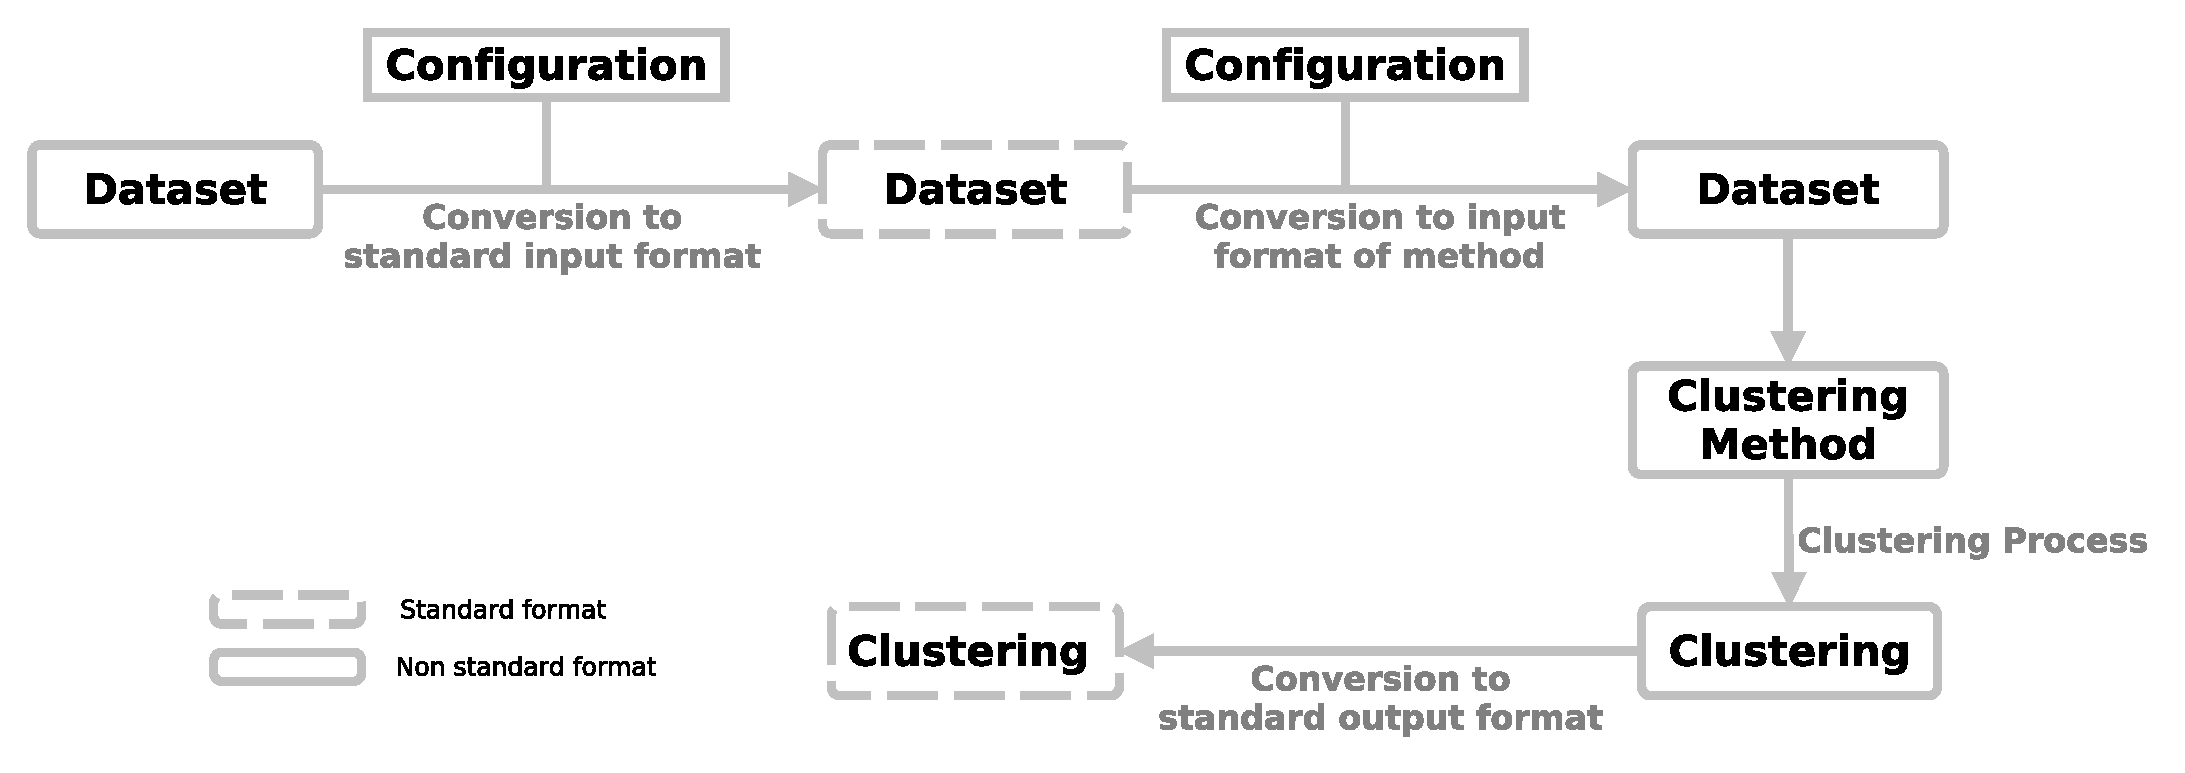
\includegraphics[width=.75\textwidth]{../master_seminar_presentation/flow_dataset.png} 
	\end{figure}

	If a new clustering method is added to the framework, its input and output formats need to be known to the framework. 
	
	\clusteval ships with a set of supported input and output formats. The input formats are
	
	\begin{itemize}
		\item APRowSimDataSetFormat
		\item BLASTDataSetFormat
		\item MatrixDataSetFormat
		\item RowSimDataSetFormat
		\item SimMatrixDataSetFormat
		\item TransClustSimMatrixDataSetFormat
	\end{itemize}
	and the output formats are
	\begin{itemize}
		\item APRunResultFormat
		\item MCLRunResultFormat
		\item TabSeparatedRunResultFormat
		\item TransClustRunResultFormat
	\end{itemize}
	
	If the new clustering method requires another input format not in the list, you will have to make it available to the framework by writing
	\begin{itemize}
		\item a wrapper class for this dataset format and 
		\item a parser, which converts the standardized input format of this framework to this input format.
	\end{itemize}
	If the new clustering method has a so far unknown output format, you will have to provide
	\begin{itemize}
		\item a wrapper class for this output format as well as
		\item a parser that converts that format to the standardized output format.
	\end{itemize}
	When this clustering method is applied to a dataset, the resulting clustering in the new format is converted to a standardized output format using your parser, such that further analyses can be performed regardless of the used clustering method.

For more information on how the framework can be extended by new input or output formats see \ref{formats} respectively.


	
			\subsubsection{Standard input format} \label{subsubsec:standarddatasetformat}
			The standard input format is a SimMatrixDataSetFormat which is described under \ref{subsubsec:simmatrixdatasetformat}.
			\subsubsection{APRowSimDataSetFormat}\label{aprowsimdatasetformat}
				This input format is used by Affinity Propagation. It is similar to the RowSimDataSetFormat, except that it accepts only numbers as ids and that it leaves out lines where id1=id2 such that it looks like this:
				\begin{lstlisting}
1	2	0.2
1	3	0.6
2	1	0.2
2	3	0.5
3	1	0.6
3	2	0.5				\end{lstlisting}
			\subsubsection{BLASTDataSetFormat}
				The BLAST dataset format needs a all-vs-all BLAST file and a corresponding FASTA file.
				
				\textbf{Please note}, that the FASTA file has to be named exactly like the BLAST file plus the additional .fasta extension. If the BLAST file is named like MyBlastFile.blast, then the FASTA file only be found by the framework, when it lies in the same directory and is named MyBlastFile.blast.fasta.
				
			\begin{lstlisting}
d1dlwa_	d1dlwa_	77.59	116	0	0	1	116	1	116	4.4e-46	172.6
d1dlwa_	d1idra_	40.30	67	40	0	19	85	31	97	3.2e-12	60.08
d1dlwa_	d1dlya_	32.00	100	62	1	19	116	19	118	1.6e-11	57.77
d1dlwa_	d2gdm__	45.45	22	12	0	60	81	89	110	0.435	23.10
d1dlwa_	d1cqxa1	37.50	24	15	0	62	85	79	102	0.969	21.94
d1dlwa_	d1cqxa1	40.00	5	3	0	71	75	134	138	4975.0	9.62
d1dlwa_	d1kr7a_	31.25	32	22	0	41	72	45	76	  4.8	19.63
d1dlwa_	d1kr7a_	50.00	8	4	0	50	57	91	98	202.0	14.24
d1dlwa_	d1kr7a_	66.67	3	1	0	50	52	86	88	6497.5	9.23
d1dlwa_	d1edg__	45.00	20	11	0	47	66	262	281	  6.3	19.25			\end{lstlisting}
				
			\begin{lstlisting}
>d1dlwa_
slfeqlggqaavqavtaqfyaniqadatvatffngidmpnqtnktaaflc
>d1dlya_
slfaklggreaveaavdkfynkivadptvstyfsntdmkvqrskqfafla
>d1idra_
gllsrlrkrepisiydkiggheaievvvedfyvrvladdqlsaffsgtnm
>d1kr7a_
mvnwaavvddfyqelfkahpeyqnkfgfkgvalgslkgnaayktqagktv\end{lstlisting}

			\subsubsection{MatrixDataSetFormat}
			This input format is a absolute dataset format, that means it contains samples together with their absolute coordinates:
			
\begin{lstlisting}
ALL_19769_B.cell	759	169	54	36
ALL_19769_B.cell_2	1062	88	235	38
ALL_28373_B.cell	822	196	150	120
ALL_28373_B.cell_2	1068	146	221	16
ALL_9692_B.cell		1455	53	217	169
\end{lstlisting}
			 

			\subsubsection{RowSimDataSetFormat}
				This input format consists of tab-separated rows looking as follows:
				\begin{lstlisting}
id1	id1	1.0
id1	id2	0.2
id1	id3	0.6
id2	id1	0.2
id2	id2	1.0
id2	id3	0.5
id3	id1	0.6
id3	id2	0.5
id3	id3	1.0				\end{lstlisting}
				
			\subsubsection{SimMatrixDataSetFormat} \label{subsubsec:simmatrixdatasetformat}
			 The SimMatrixDataSetFormat is a complete quadratic tab-separated similarity matrix with header row and column (containing ids). A dataset file with the SimMatrixDataSetFormat could look as follows:
			\begin{lstlisting}
	id1	id2	id3
id1	1.0	0.2	0.6
id2	0.2	1.0	0.5
id3	0.6	0.5	1.0
\end{lstlisting}
			There are no spaces in this file, only tabs. It does not necessarily need to be symmetric, it depends on the clustering method, whether it supports asymmetric similarity data.
			
			\subsubsection{TransClustSimMatrixDataSetFormat}
			This format can be used by Transitivity Clustering and it looks as follows:
			\begin{lstlisting}
3	
id1
id2
id3
0.2	0.6
0.5
\end{lstlisting}

	The number in the first line is the number of ids. It is followed by all ids in the next lines. Then it follows the tab-separated upper half of the similarity matrix. This format expects that the similarity matrix is symmetric.
	

		\subsubsection{Standard output format} \label{subsubsec:standardrunresultformat}
		The standard output format contains one clustering generated for parameter values $p_1=v1$,...,$p_K=vK$ in one line with clusters $c1,...,cK$, cluster sizes $size(ci) = si$. Every cluster $ci$ contains elements $e\_i\_1,...,e\_i\_si$ with fuzzy coefficients $f\_i\_1,...,f\_i\_si$. The format for this looks as follows:
		
		\begin{verbatim}
p1,...,pK	Clustering
v1,...,vK	e_1_1:f_1_1,...,e_1_s1:f_1_s1;...;e_K_1:f_K_1,...,e_K_sK:f_K_sK
	\end{verbatim}
	
	The parameter names and values on the left have to be separated by a TAB from the string "Clustering" and the clustering on the right. If the fuzzy coefficients are missing, the framework will not be able to parse the result file.
		
		\subsubsection{APRunResultFormat}
		This is the result format of Affinity Propagation.
		\subsubsection{MCLRunResultFormat}
		This is the result format of Markov Clustering.
		\subsubsection{TransClustRunResultFormat}
		This is the result format of Transitivity Clustering.
		

	\subsection{Clustering Quality Measures}\label{clustQualMeasures}
	The clustering quality measures are used by the framework to assess the quality of calculated clusterings. \clusteval ships with a standard set of clustering quality measures
	\begin{itemize}
		\item F1 \& F2-Score
		\item False Discovery Rate (FDR)
		\item False Positive Rate (FPR)
		\item Rand Index
		\item Sensitivity
		\item Specificity
		\item Silhouette Value (Java \& R implementation)
	\end{itemize}
	Please check \ref{clustQualMeasures} for more information on how to extend the framework by new clustering quality measures.
	\subsection{Distance Measures}\label{distanceMeasures}
	 The distance measures are used when converting absolute datasets (containing absolute coordinates) to relative datasets (pairwise similarities). The distance measures define how to assess the similarity between a pair of objects given their absolute coordinates.
	\clusteval ships with the following distance measures
	\begin{itemize}
		\item Euclidian
		\item Hoeffding D Statistic$^{(Rserve)}$
		\item Pearson Correlation Coefficient$^{(Rserve)}$
		\item Spearman Correlation Coefficient$^{(Rserve)}$
	\end{itemize}
	Please check \ref{distanceMeasures} for more information on how to extend the framework by new distance measures.
	\subsection{Parameter Optimization Methods}\label{paramOptMethods}
	 The backend can perform automatized and autonomous optimization of parameters of clustering methods. This is an iterative procedure where the backend assesses qualities of clustering results of the last iteration and adapts the parameter for the next iteration in order to find optimal parameters for the method on the given data. The parameter optimization method determines the following aspects:

\begin{enumerate}
\item the number of iterations of the optimization process
\item the parameter sets evaluated
\item the handling of diverging iterations
\item the storage of the iteration results in RAM
\end{enumerate}


	\clusteval ships with the following set of parameter optimization methods
	\begin{itemize}
		\item Affinity Propagation Divisive Parameter Optimization Method
		\item Affinity Propagation Parameter Optimization Method
		\item Divisive Parameter Optimization Method
		\item Gap Statistic Parameter Optimization Method
		\item Layered Divisive Parameter Optimization Method
		\item Transitivity Clustering Parameter Optimization Method
		\item Transitivity Clustering Quantile Parameter Optimization Method
	\end{itemize}
	Detailed information about each of these methods can be found in \cite{wiwie_2013}. Please check \ref{paramOptMethods} for more information on how to extend the framework by new parameter optimization methods.
	

	
	\subsection{Configuration Files}
	Above we already discussed that the framework needs \textbf{program configurations}, \textbf{dataset configurations} and \textbf{goldstandard configurations}. Those configuration files directly reference corresponding files (dataset, goldstandard, \ldots) on the filesystem. Internally the framework has some abstraction layers to store all the configurations. Figure \ref{fig_backend_configurations} shows the overall abstractional structure of the configuration files used in the backend. One can see that dataset- and goldstandard configuration are linked together in a \textbf{data configuration}.
	
	A run is an abstract entity that can be performed by the backend. Its execution involves (in most cases) application of clustering methods to several datasets, and afterwards clustering qualities are assessed using the goldstandards corresponding to each dataset. A run corresponds to a \textbf{run configuration} file, which then again references the \textbf{program-} and \textbf{data configurations} that should be pairwise combined.
	
	When a run is performed by the backend, the clustering methods wrapped by all referenced program configurations are applied to all datasets indirectly referenced through the data configurations.
	
	
	\begin{figure}[hbtp]
	\caption{Backend Configurations}
	\label{fig_backend_configurations}
	\centering
	\includegraphics[width=.75\textwidth]{../master_seminar_presentation/backend_configurations.png} 
	\end{figure}
	

	
		\subsubsection{Data Configurations} \label{subsec:dataconfigs}
		A data configuration is a file, that combines two other configurations together: A dataset configuration (see \ref{subsubsec:datasetconfigs}) and a goldstandard configuration (see \ref{subsubsec:gsconfigs}). Later on when you create a run (and its configuration) and in this run you want to apply two clustering methods to three datasets (together with their goldstandards) you will do so by telling the run configuration the names of the three corresponding data configurations. \textbf{Please note:} The data configuration file has to have the file extension .dataconfig, otherwise it will not be recognized by the framework.
		\begin{description}
		\item[datasetConfig:]
			This option has to be set to the name of the dataset configuration (see \ref{para:datasetName}), \textit{not} the name of the file.
			
		\item[goldstandardConfig:]
			This option has to be set to the name of the goldstandard configuration (see \ref{para:goldstandardName}), \textit{not} the name of the file.
		\end{description}
			
		\subsubsection{Example Data Configuration} A data configuration could like as follows:
\begin{listing}{1}
datasetConfig = astral_1
goldstandardConfig = astral_1_161\end{listing}


		
			\subsubsection{Dataset Configuration} \label{subsubsec:datasetconfigs}
			A dataset configuration tells the framework meta information about the corresponding dataset. That is: The internal name of the dataset, its filename and its format.
			
			\begin{description}
			\item[datasetName:] \label{para:datasetName}
			This name is used to find and access datasets within the framework. The name of the dataset \textit{has} to be identical to the subfolder of the corresponding dataset.
			\item[datasetFile:] \label{para:datasetFile}
			This option has to be set to the filename of the dataset file residing within the subfolder of the dataset.
			\item[datasetFormat:] \label{para:datasetFormat}
			This option tells the framework, which format the dataset is in. \clusteval ships with a set of supported dataset formats. Please note, that the entries in this list \textit{have} to be identical with the simple names of the corresponding dataset format classes.
			\item[[distanceMeasureAbsoluteToRelative:]] This indicates, which distance measure should be used, when this dataset is converted to another format. Defaults to EuclidianDistanceMeasure.
			\item[[preprocessorAfterDistance:]]A comma seperated list of data
				 preprocessors to apply, before the data is converted to pairwise
				 similarities (the standard input format)
			\item[[preprocessorAfterDistance:]] A comma seperated list of data
				 preprocessors to apply, after the data is converted to pairwise
				 similarities (the standard input format)
			\end{description}
	
			\subsubsection{Example Dataset Configuration}
			
			\begin{listing}{1}
datasetName = astral_1_161
datasetFile = blastResults.txt
datasetFormat = BLASTDataSetFormat
distanceMeasureAbsoluteToRelative = EuclidianDistanceMeasure \end{listing}

			\subsubsection{GoldStandard Configuration} \label{subsubsec:gsconfigs}
			A goldstandard configuration tells the framework meta information about the corresponding goldstandard. That is: The internal name of the goldstandard and its filename.
			
			\begin{description}
			\item[goldstandardName:] \label{para:goldstandardName}
			This name is used to find and access goldstandards within the framework. The name of the goldstandard \textit{has} to be identical to the subfolder of the corresponding goldstandard.
			\item[goldstandardFile:] \label{para:goldstandardFile}
			This option has to be set to the filename of the goldstandard file residing within the subfolder of the goldstandard.
			\end{description}
	
			\subsubsection{Example Goldstandard Configuration}
			
			\begin{listing}{1}
goldstandardName = astral_1_161
goldstandardFile = astral_161.goldstandard_3.txt \end{listing}
			
	

		\subsubsection{Program Configurations} \label{subsec_programconfigs}
		For every clustering method there can be several configuration files. All program configurations have to be located in \highlight{\repoprogramconfigs}. A program configuration tells the framework, what parameters the program expects, how to invoke the executable, with what parameter values to invoke it and several other information. Possible entries in a program configuration follow.
		
		\textbf{Please note:} The program configuration file has to have the file extension \highlight{.config}, otherwise it will not be recognized by the framework.
		
	\begin{description}
		\item[type:] Indicates, whether the program described by this program configuration is a standalone or an R program. This option can be set to either \textit{standalone} or the simple name of the R program class.

		\item[program:] This is the full name of the clustering method, this configuration references. When a clustering method is located in \highlight{\repoprograms/some/program}, then the full name of the program is "some/program"
		
		\item[alias:] This option is only interpreted for standalone programs. It tells the framework a alias of the corresponding program, which is used whenever the program needs to be represented in a readable format, e.g. on the website.
		
		\item[parameters:] 	A comma-separated list of parameters the program uses and which can be used when the program is invoked. These parameters need to be set to valid values before the program is actually applied to a dataset. Parameter values can be specificely defined either in a program or run configuration or, in case of parameter optimization runs, they are autonomously determined by the framework. If no value is defined for a program parameter at all, it will be set to its default value given in the program configuration.
		
		\item[optimizationParameters:] This option is only used, when a run is performed in parameter optimization mode. Then this list of parameters (that needs to be a subset of the list given in option "parameters") is used to determine, which parameters can be in principle optimized when this program is used in parameter optimization mode.
		
		\item[compatibleDataSetFormats:] This list tells the framework, which input formats this program supports. Please note, that the entries in this list \textit{have} to be identical to the simple names of the classes of the corresponding dataset formats.
		
		\item[outputFormat:] This option tells the framework, what the output format of this program is. Please note, that the naming convention of this list follows the same rules as those of "compatibleDataSetFormats", as the value of this option has to be named exactly after the simple name of the corresponding class.
		
		\item[expectsNormalizedDataSet:] This option can be set to "true" or "false". By default, it is set to false. If you set it to true, the input similarities (only) for this program are normalized to values between 0 and 1. This may help you, if a clustering method does not support negative values or values outside certain ranges.
		
		\item[[invocationFormat]] This is the section containing a set of invocation formats which tell the framework in string format, how to invoke this program. The invocation formats may contain program parameters or certain predefined variables, which are replaced by the framework during runtime. Such variable names are enclosed by \% signs. All program parameters defined in the parameters section of the program configuration can be used in the invocation format string. Additionally the following variables are hardcoded for every program and cannot be used for other parameters:
			\begin{description}
				\item[\%e\%] will be replaced by the absolute path of the executable
				\item[\%i\%] will be replaced by the absolute path of the input
				\item[\%o\%] will be replaced by the absolute path of the output
				\item[\%gs\%] will be replaced by the absolute path of the goldstandard
			\end{description}
			
			For example, if the option is set like this:
			
				\code{invocationFormat = \%e\% \%i\% \%preference\% \%o\% maxits=\%maxits\% convits=\%convits\%}
				
			"preference", "maxits" and "convits" have to be defined in the "parameters" entry of the same program configuration.
			
	\begin{description}
		\item[invocationFormat:]
			This is the option which tells the framework, how to invoke this program in case we have a goldstandard and no parameter optimization run. All words enclosed with \% will be replaced by the framework at runtime. All other variables in the invocation line have to be parameters defined in this program configuration.
			
		\item[invocationFormatWithoutGoldStandard:]
			This is how to invoke this program in case we have no goldstandard and no parameter optimization run.
			
		\item[invocationFormatParameterOptimization:]
			This is how to invoke this program in case we have a goldstandard and a parameter optimization run.
			
		\item[invocationFormatParameterOptimizationWithoutGoldStandard:]
			This is how to invoke this program in case we have no goldstandard and a parameter optimization run.
		\end{description}
		\item[[$<$parameterName$>$]]
			For every parameter defined in the list of entry "parameters", there needs to be an additional section in the program configuration, which tells the framework several information about the parameter:
			\begin{description}
				\item[desc:] A description of the parameter
				\item[type:] One of the types FLOAT ("2"), INTEGER ("1") or STRING ("0").
				\item[def:] A default value for the parameter.
				\item[minValue:] The minimal value for the parameter.
				\item[maxValue:] The maximal value for the parameter.
			\end{description}
	\end{description}
			
		\subsubsection{Example program configuration}
		%\fontsize{10pt}{12pt}
		\begin{listing}{1}
program = APcluster
parameters = preference,maxits,convits,dampfact
optimizationParameters = preference,maxits,convits,dampfact
executable = apcluster
compatibleDataSetFormats = APRowSimDataSetFormat
outputFormat = APRunResultFormat

[invocationFormat]
invocationFormat = %e %i %preference %o maxits=%maxits convits=%convits 
dampfact=%dampfact

[maxits]
desc = Max iterations
type = 1
def = 2000
minValue = 2000
maxValue = 5000

[convits]
desc = Cluster Center duration
type = 1
def = 200
minValue = 200
maxValue = 500

[dampfact]
type = 2
def = 0.9
minValue = 0.7
maxValue = 0.99

[preference]
desc = Preference
type = 2
def = 0.5
minValue = 0.0
maxValue = 1.0		\end{listing}


	
	\subsection{Runs} \label{sec:runs}

\begin{figure}[hbtp]
\caption{Inheritance of different run types}
\label{fig_run_inheritance}
\centering
\includegraphics[width=.6\textwidth]{../master_seminar_presentation/run_inheritance.png}
\end{figure} 
	
		Runs are entities that can be performed by the backend server. A run is defined by a file in the folder \highlight{\reporuns}. The name of that file (without extension) also defines the name of the run. Depending on the type of the run this file contains several other components which configure the process when the run is performed. Figure \ref{fig_run_inheritance} shows the different types of runs and how they relate to each other.
		
		\subsubsection{Run Files} \label{run_files}
		
		Every run is defined in a run-file in the corresponding folder of the repository. Depending on the type of the run, different options are available that can be specified in the run-file. Common to all types of runs are the following options:
		
		\begin{description}
			\item[mode:] \label{subsubsec:runconfigmode}
				This entry can be set to "clustering",  "parameter\_optimization", "dataAnalysis", "runAnalysis" or "runDataAnalysis". These types can be found in the aforementioned figure and are described in the following paragraphs.
		\end{description}
		
		\subsubsection{Execution Runs} \label{execution_runs}		
			Execution runs calculate clusterings during their execution and assess qualities for every of those clusterings. Clusterings are calculated by applying clustering methods to datasets using a certain parameter set. That is why execution runs have sets of both, program and data configurations. During execution time every program configuration is applied to every data configuration in a pairwise manner. For every calculated clustering a set of clustering quality measures are assessed.
			
		  In general the options of such a combination of data and program configuration will be taken from these configurations respectively, but can be overridden by the options in the run configuration, That means parameter values defined in the program as well as in the run configuration will be taken from the latter.
		 
		 \subsubsection{Execution Run Files}\label{execution_run_files} For execution runs, additionally to the options defined for all runs (see \nameref{run_files}), the following options for the run-file are defined:
		 \begin{description}
			\item[programConfig:]
			This entry has to be set to a single name or a comma-separated list of names of program configurations. When this run is performed, these program configurations will be pairwise combined with the data configurations given in the option "dataConfig". 
			\item[dataConfig:]
			This entry has to be set to a single name or a comma-separated list of names of data configurations. When this run is performed, these data configurations will be pairwise combined with the program configurations given in the option "programConfig". 
			\item[qualityMeasures:] \label{subsubsec:runconfigqualmeasure}
				This option determines, which quality measures will be assessed for every clustering calculated during the run process. When this run is a clustering run (see option "mode"), then for every pair of data and program configurations there will be only one clustering as a result for which quality measures will be evaluated. When the mode is set to "parameter\_optimization", for every iteration during the parameter optimization process these quality measures will be evaluated.
			\item[[$<$programConfigName$>$]:]
			If a dedicated section is found in this run file that is called like one of the program configurations given in option "programConfig", several parameters can be overridden individually only for this program configuration which are
			\begin{description}			 	
				\item[$<$parameterName$>$:] The program parameter with the given name which needs to be defined in the program configuration can be fixed to a certain value.
\end{description}
		 \end{description}
		  
		 \subsubsection{Clustering Runs}\label{clustering_runs}
		 Clustering runs are a type of execution run, that means they calculate clusterings by applying every program configuration to every data configuration. Afterwards they assess the qualities of those clusterings in terms of several clustering quality measures.
		 
		 In the case of clustering runs for every pair of program and data configuration exactly one clustering is calculated and assessed. Clustering runs are visualized in figure \ref{clustering_run_process}.
		 
		 \begin{figure}[hbtp]
		 \caption{Clustering Run Process}
		 \label{clustering_run_process}
		 \centering
		 \includegraphics[width=\linewidth]{../master_seminar_presentation/framework_flow_singleclustering.png}
		 \end{figure}
		 
		 \paragraph{Clustering Run File} For clustering runs, the options are the same as for all execution runs (see \nameref{execution_run_files}).
		 
		  
		 \subsubsection{Parameter Optimization Runs}\label{paramOpt_runs}
		 Parameter optimization runs are a type of execution run, that means they calculate clusterings by applying every program configuration to every data configuration. Afterwards they assess the qualities of those clusterings in terms of several clustering quality measures.
		 
		In contrast to clustering runs, parameter optimization runs calculate several clusterings for every pair of data and program configuration in a pairwise manner. Every clustering corresponds to a certain parameter set and the parameter sets to evaluate are determined by a parameter optimization method (see \ref{paramOptMethods} for more information). Parameter optimization runs are visualized in figure \ref{paramOpt_run_process}.
		
		\begin{figure}[hbtp]
		\caption{Parameter Optimization Run Process}
		\label{paramOpt_run_process}
		\centering
		\includegraphics[width=\linewidth]{../master_seminar_presentation/framework_flow_parameterOptimization.png}
		\end{figure}
		
		\paragraph{Parameter Optimization Run File}\label{paramOpt_run_files}
		
		For parameter optimization runs, additionally to the options defined for all execution runs (see \nameref{execution_run_files}), the following options for the run-file are defined:
		 \begin{description}
		 	\item[optimizationMethod:] The parameter optimization method to use when this run is performed.
		 	\item[optimizationCriterion:] The clustering quality measure which should be used as optimization criterion. This criterion is used to determine the optimal parameter set during the optimization process. Therefore it can influence the cause of the optimization process, if the chosen parameter optimization method integrates the qualities of previous iterations into future iterations.
		 	\item[optimizationIterations:] The number of total optimization iterations that should be performed for every pair of program and data configuration. \textbf{Hint:} This number might not be the number, the optimization process performs in the end, since it gives only a desirable number that might not be accurately realizable for a specific optimization method.
			\item[[$<$programConfigName$>$]:]
			If a dedicated section is found in this run file that is called like one of the program configurations given in option "programConfig", several parameters can be overridden individually only for this program configuration which are
			\begin{description}			 	
				\item[optimizationParameters:] A comma separated list of the parameters that should be optimized for this program configuration
				\item[optimizationMethod:] The parameter optimization method to use for this program configuration
\end{description}
		 \end{description}
		
		
		\subsubsection{Analysis Runs} \label{analysis_runs}		
			Analysis runs assess certain properties of objects of interest. An analysis run has a set of target objects and a set of statistics, that should be assessed for each of the target objects. That means, during execution time for every target object every statistic is assessed in a pairwise manner.
		
		\subsubsection{Data Analysis Runs} \label{dataAnalysis_runs}		
			In case of data analysis runs the target objects to analyze are data configurations (indirectly datasets) and the statistics are data statistics, that is properties of datasets. Data analysis runs are visualized in figure \ref{dataAnalysis_run_process}.
		
		\begin{figure}[hbtp]
		\caption{Data Analysis Run Process}
		\label{dataAnalysis_run_process}
		\centering
		\includegraphics[width=\linewidth]{../master_seminar_presentation/framework_flow_dataAnalysis.png}
		\end{figure}
		
		\subsubsection{Data Analysis Run File}\label{dataAnalysis_run_file}

		For data analysis runs the following options for the run-file are defined:
		 \begin{description}
		 	\item[dataStatistics:] A comma separated list of data statistics to assess for the given data configurations.
		 	\item[dataConfig:] A comma separated list of data configurations to analyse.
		 \end{description}
			
		
		\subsubsection{Run Analysis Runs} \label{runAnalysis_runs}		
			In case of run analysis runs the target objects to analyze are clusterings (results of execution runs) and the statistics are run statistics, that is properties of execution run results. Run analysis runs are visualized in figure \ref{runAnalysis_run_process}.
		
		\begin{figure}[hbtp]
		\caption{Run Analysis Run Process}
		\label{runAnalysis_run_process}
		\centering
		\includegraphics[width=\linewidth]{../master_seminar_presentation/framework_flow_runAnalysis.png}
		\end{figure}
		
		\subsubsection{Run Analysis Run File}\label{runAnalysis_run_file}

		For run analysis runs the following options for the run-file are defined:
		 \begin{description}
		 	\item[runStatistics:] A comma separated list of run statistics to assess for the given execution run results.
		 	\item[uniqeRunIdentifiers:] A comma separated list of identifiers of execution run results. See \ref{runresults} for an explanation on run result identifiers.
		 \end{description}
		
		\subsubsection{Run-Data Analysis Runs} \label{runDataAnalysis_runs}		
			In case of run-data analysis runs the target objects to analyze are pairs of data configurations and clusterings (results of execution runs) and the statistics are run-data statistics, that is relationships between execution run results and properties of data configurations. Run-Data analysis runs are visualized in figure \ref{runDataAnalysis_run_process}.
		
		\begin{figure}[hbtp]
		\caption{Run-Data Analysis Run Process}
		\label{runDataAnalysis_run_process}
		\centering
		\includegraphics[width=\linewidth]{../master_seminar_presentation/framework_flow_runDataAnalysis.png}
		\end{figure}
		
		\subsubsection{Run-Data Analysis Run File}\label{runDataAnalysis_run_file}

		For run-data analysis runs the following options for the run-file are defined:
		 \begin{description}
		 	\item[runDataStatistics:] A comma separated list of run-data statistics to assess for every pair of given execution run result and data analysis result.
		 	\item[uniqeRunIdentifiers:] A comma separated list of identifiers of execution run results. See \ref{runresults} for an explanation on run result identifiers.
		 	\item[uniqeDataIdentifiers:] A comma separated list of identifiers of data analysis run results. See \ref{runresults} for an explanation on run result identifiers.
		 \end{description}
			
			\subsubsection{Examples of a Run Configurations}
			
			See \ref{fig:runconfig1} and \ref{fig:runconfig2} for examples of run configuration files.
			
			\begin{figure}[hbtp]
			\label{fig:runconfig1}
			\caption{Example run configuration "all\_vs\_astral\_1\_171.runconfig" for Parameter Optimization Mode}
			\begin{lstlisting}
programConfig = APcluster_1,TransClust_2,MCL_1
dataConfig = astral_1_171
qualityMeasures = TransClustF2ClusteringQualityMeasure,SilhouetteValueRClusteringQualityMeasure
mode = parameter_optimization
optimizationMethod = DivisiveParameterOptimizationMethod
optimizationCriterion = SilhouetteValueRClusteringQualityMeasure
optimizationIterations = 1001

[TransClust_2]
optimizationParameters = T

[MCL_1]
optimizationParameters = I

[APcluster_1]
optimizationParameters = preference,dampfact,maxits,convits
optimizationMethod = APDivisiveParameterOptimizationMethod\end{lstlisting}
			\end{figure}
			
			\begin{figure}[hbtp]
			\label{fig:runconfig2}
			\caption{Example run configuration "mcl\_1.runconfig" for Clustering mode}
			\begin{lstlisting}
programConfig = MCL_1
dataConfig = DS1,test50

[MCL_1]
I = 2.0			\end{lstlisting}
			\end{figure}
			
	\subsection{Run Results}\label{runresults}

	When a run is performed, a unique run identifier is determined which includes the starttime and date and the name of the run. If the run \highlight{exampleRun} is performed at the 5th of July 2012 at 12:58:38, its unique run identifier is \highlight{06\_05\_2012-12\_58\_38\_exampleRun} which is also used as the subfolder to store its results in
	
	\highlight{\reporesults/06\_05\_2012-12\_58\_38\_exampleRun}
	
	Every such folder contains some subfolders. Common to all run types are the following subfolders:
	
	\subsubsection{All run result} folders contain the following subfolders:
	
	\begin{description}
		\item \highlight{\reporesultconfigs}: Contains the configuration files that are used in this run, which includes all data-, dataset-, goldstandard- and program configurations as well as the run file.
		\item \highlight{\reporesultinputs}: Contains backups of all the input files used in this run, which includes all datasets referenced by the data configurations.
		\item \highlight{\reporesultgs}: Contains backups of all the goldstandard files used in this run.
		\item \highlight{\reporesultlogs}: Contains different log filesm, one for the complete run and one for every iteration performed during the run.
	\end{description}
	
	Depending on the run type there are additional subfolders:
	
	\subsubsection{Execution run result} folders additionally contain the following subfolders:
	
	\begin{itemize}
		\item \highlight{\reporesultcluster}
	\end{itemize}
	
	\subsubsection{Analysis run result} folders additionally contain the following subfolders:
	
	\begin{itemize}
		\item \highlight{\reporesultanalyses}
	\end{itemize}
	